
\label{Chapter:2}

\section{LArTPCs in Neutrino Physics}
Among a wide variety of detector technologies, liquid argon time projection chambers (LArTPCs) present a set of characteristics particularly interesting to neutrino physics. 
In a more general form, time projection chambers were first proposed by Nygren in 1974 \cite{Nygren}. They consist of a volume filled with a sensitive gas or liquid in a strong electrical field. When a charged particle passes through the active volume of the detector, the material is ionized, leaving a trail of ionization electrons. In the presence of an electric field, this ionization charge drifts towards charge sensitive electronics.
In the case of LArTPCs, the charge sensitive electronics consist of a set of at least two wire planes. In the first few planes, the passing of the ionization electrons through the wires produces an induction signal. In the last set of wires, the electrons are captured, producing a current, as shown in figure \ref{lartpc}. Combining information from the sets of wires and using a light trigger to calculate the drift time of the electrons in the event, it is possible to have a three dimensional calorimetric reconstruction of the track, as shown in figure \ref{lartpc_readout}. Alternatively, some experiments use the beam clock as trigger, without any light collection system. 
%
\begin{figure}[h!]
	\begin{center}
		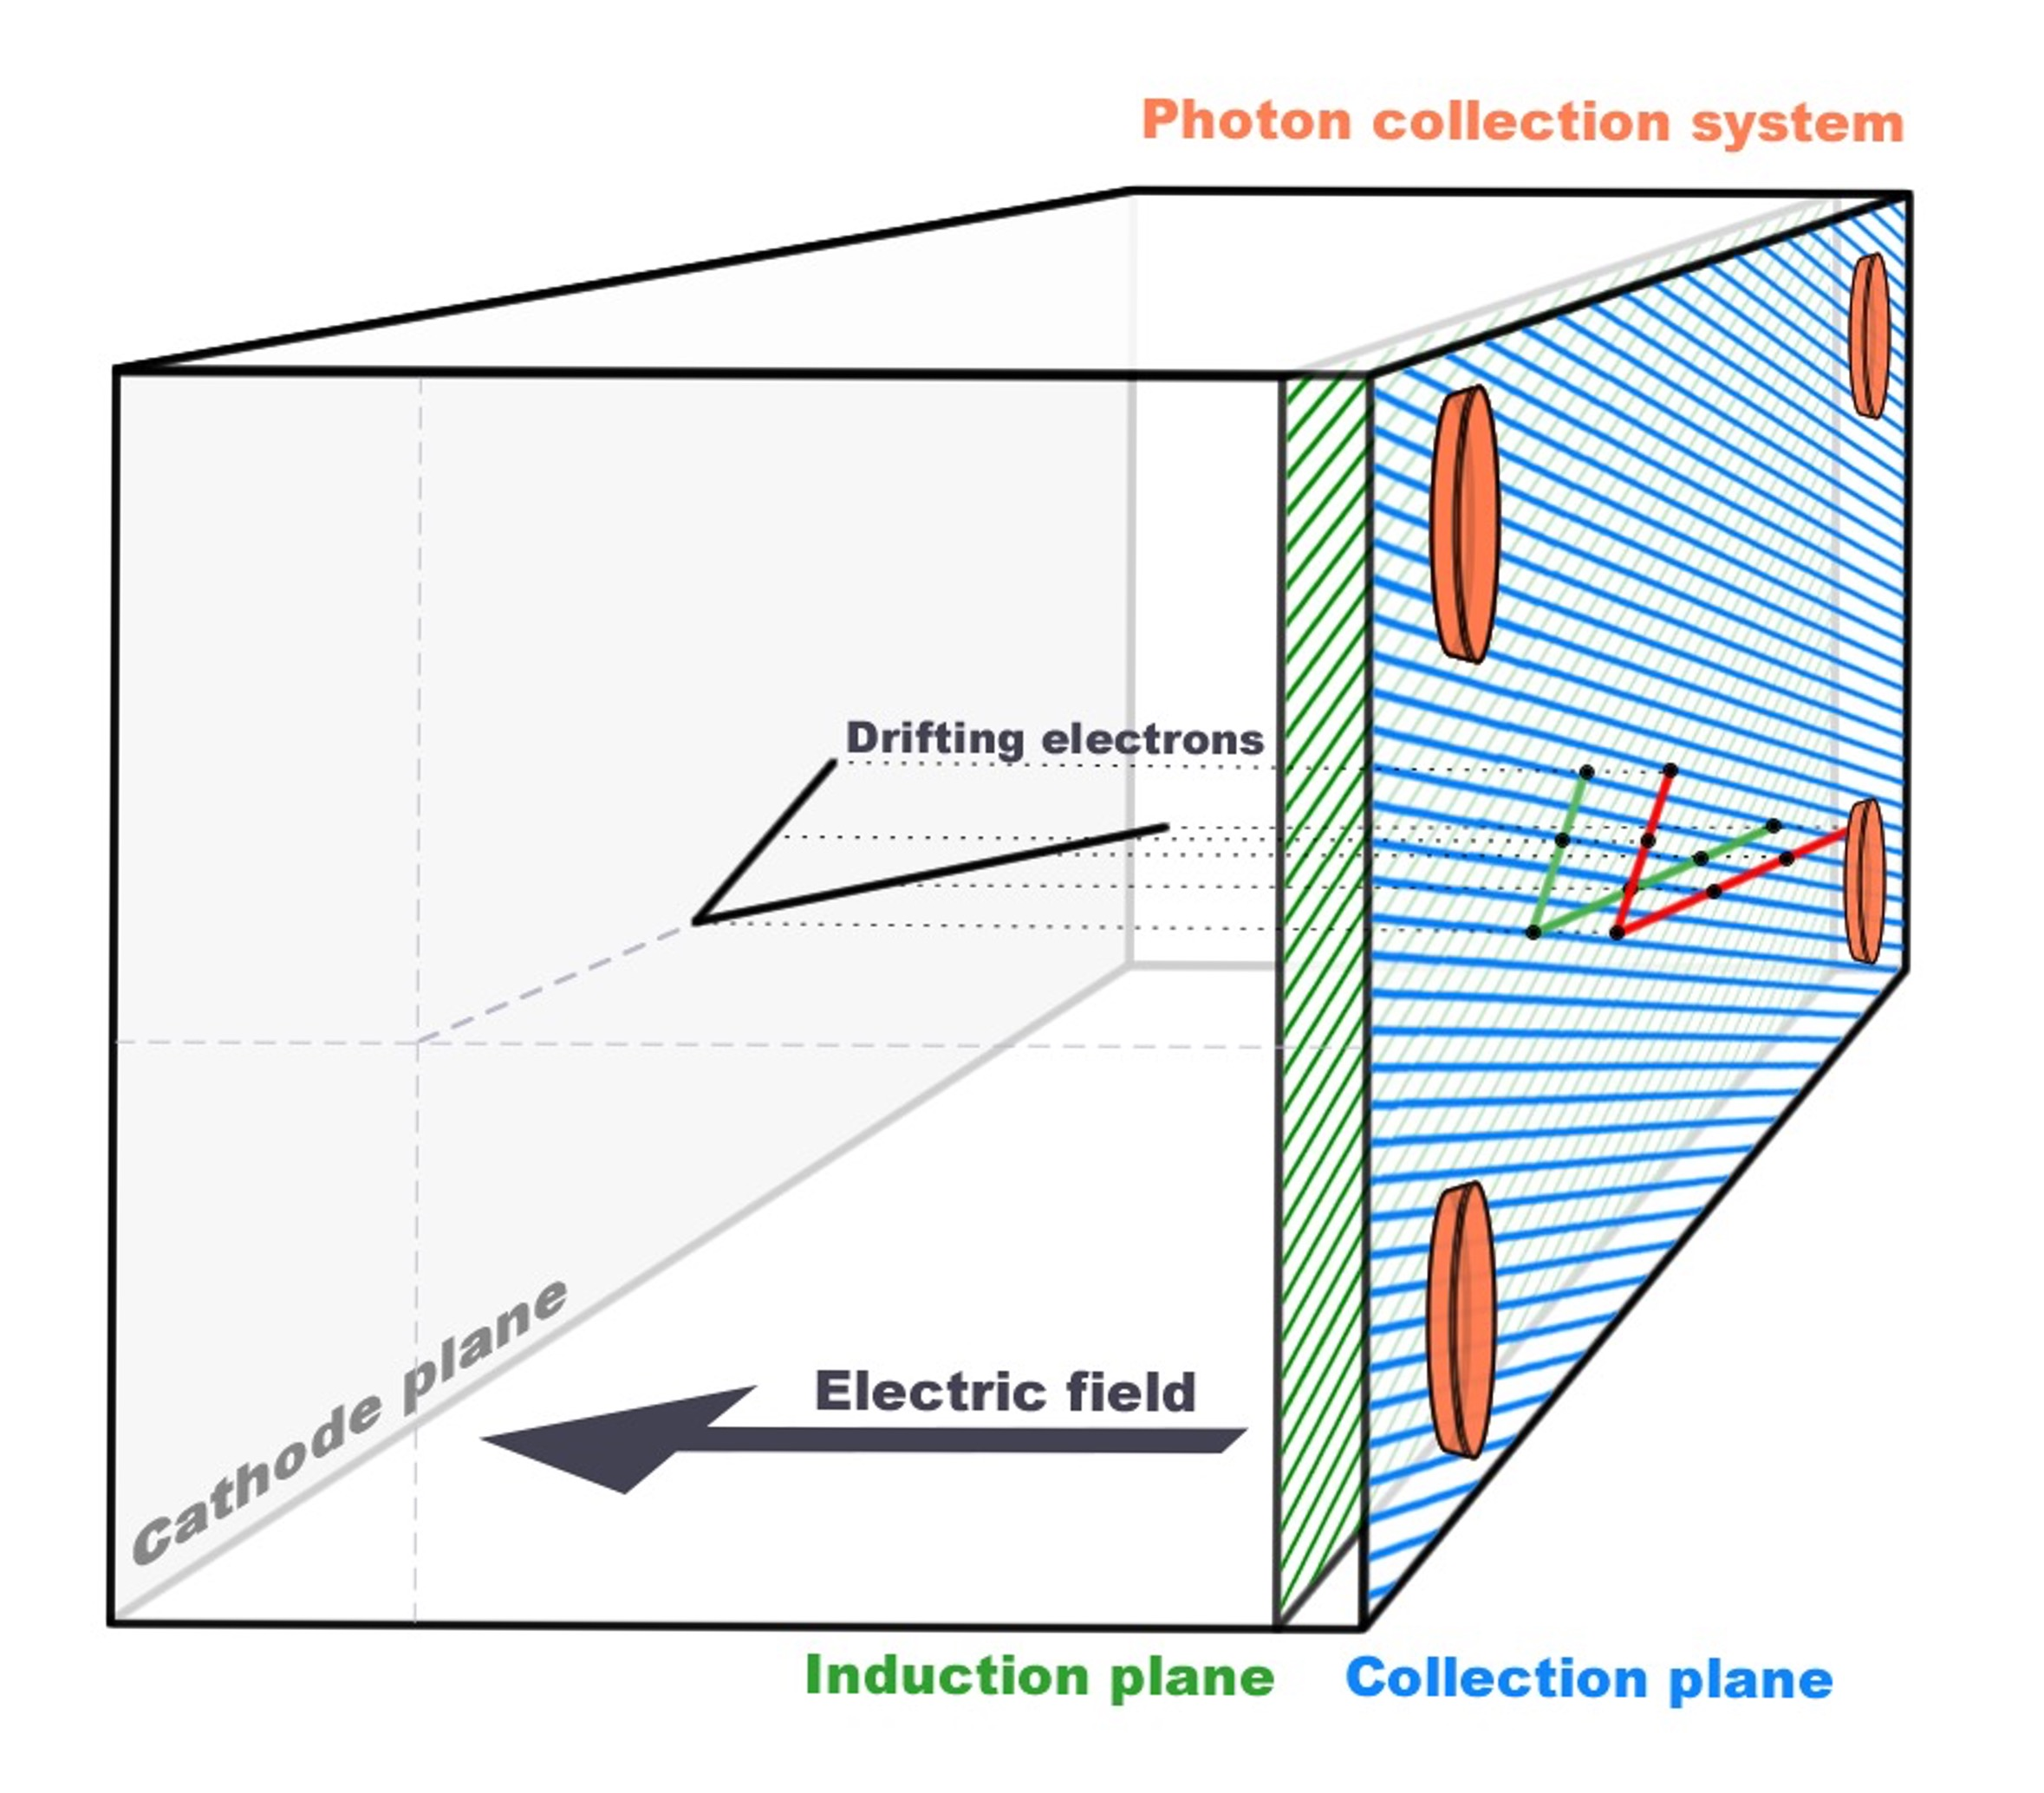
\includegraphics[scale=0.12]{Figures/LARTPC.jpg}
		\caption[LArTPC]{ {\textbf{Liquid Argon Time Projection Chamber}} \\ liquid argon time projection chambers. When a particle passes through its fiducial volume and interacts with the liquid argon, ionization electrons and scintillation light are produced. The electric field drifts the electrons from where they are produced towards the planes of wires (right corner in the figure). Both charge and light produced are read by precision wires and a light collection system (in the figure, the orange bodies behind the wires), respectively.}
		\label{lartpc}	
	\end{center}
\end{figure}
%
\begin{figure}[h!]
	\begin{center}
		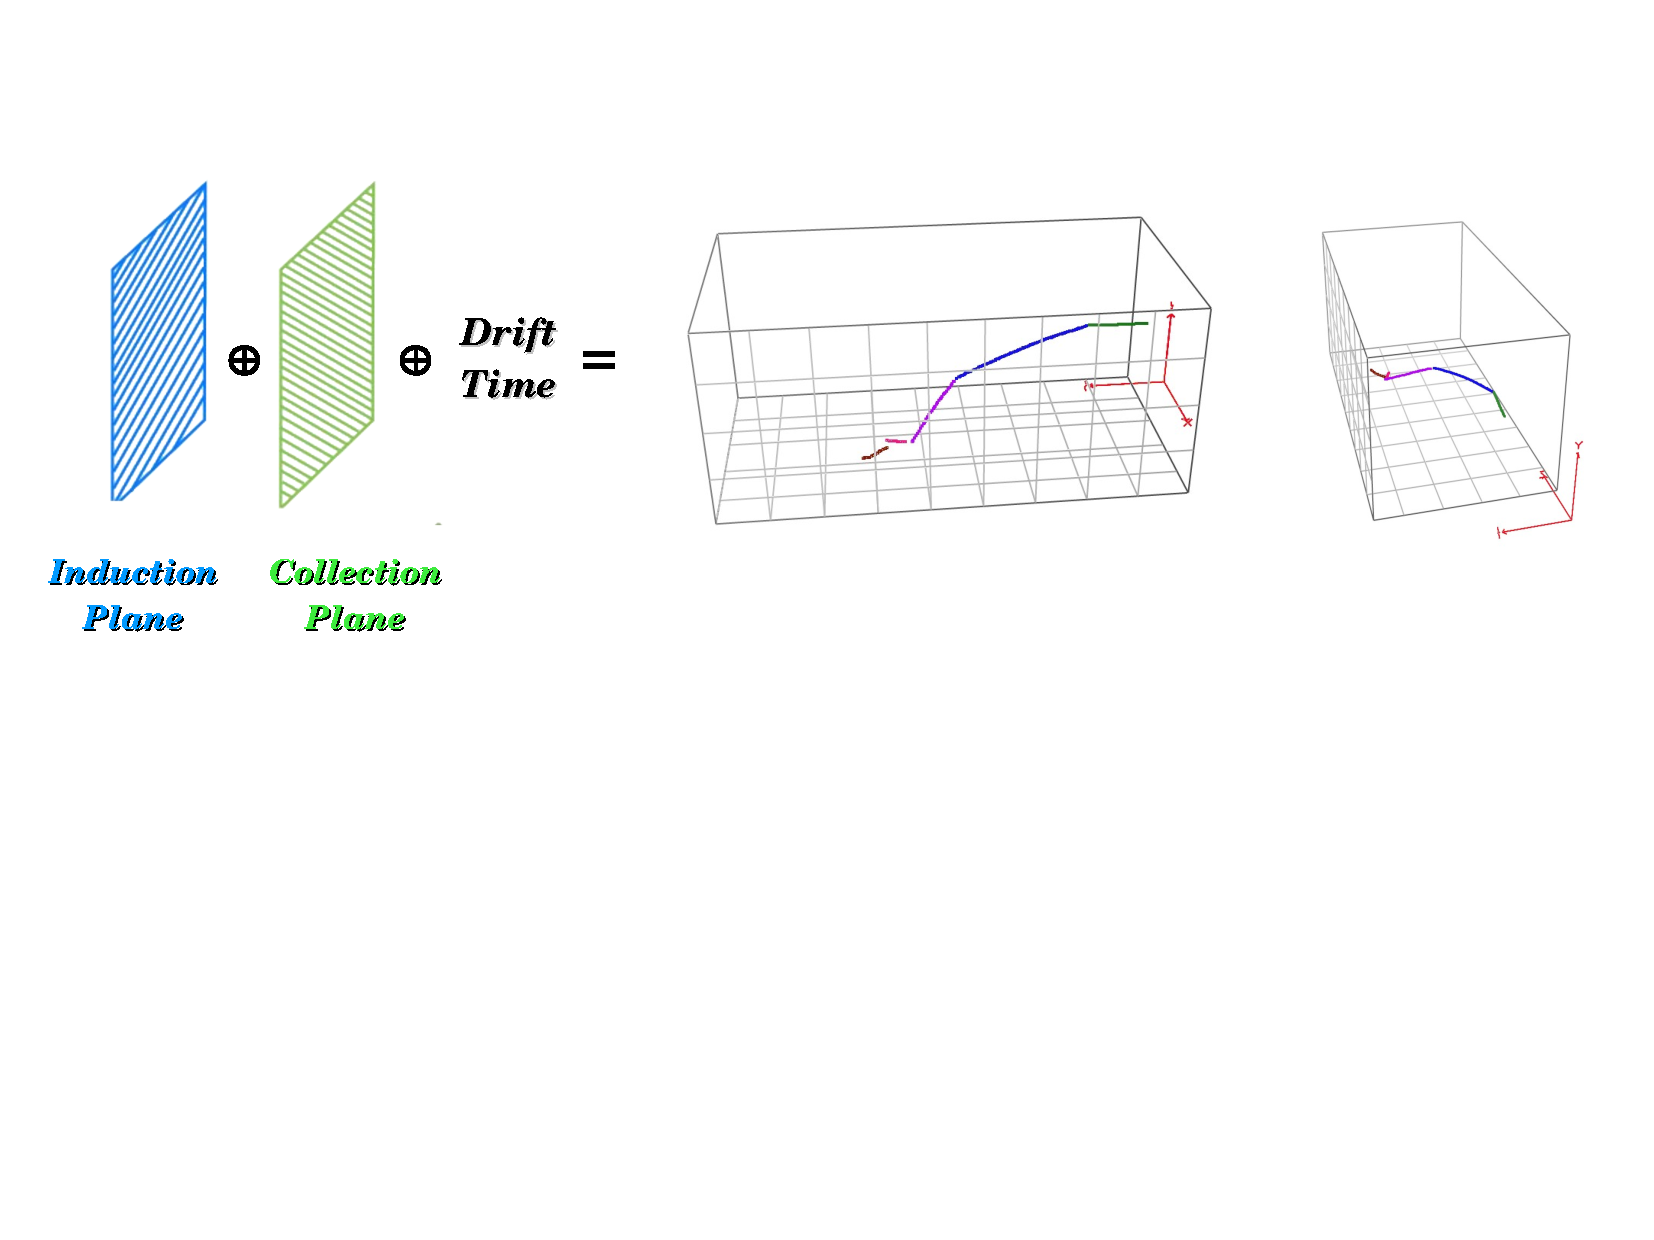
\includegraphics[scale=0.6]{Figures/Acciarri_fig2.pdf}
		\caption[LArTPC read out system]{ {\textbf{LArTPC read out system}} \\ Basic elements of the LArTPC read out system. It is needed a minimum of one induction wire plane, one collection wire plane and a light detection system. The information retrieved by those 3 components allow a 3D track reconstruction \cite{Acciarri_presentation}.}
		\label{lartpc_readout}	
	\end{center}
\end{figure}

\newpage
In 1977, not long after Nygren's proposal, Carlo Rubia noted that using liquid argon (LAr) as active material in a TPC was particularly advantageous for neutrino physics, since:
\begin{itemize}
	\item it is dense (1.4 g/cm$^3$), which increases the interaction probability;
 	\item it does not attach electrons, allowing long drift distances, which allows the construction of big detectors;
  	\item it has a high electron mobility;
   	\item argon is the third most abundant gas in the atmosphere, it is easy to obtain and purify, making it relatively cheap;
  	\item it is inert and and can be liquified with liquid nitrogen \cite{Rubia_ANewConcept}
\end{itemize}
Addicionaly, LAr is transparent to its own scintillation light. 
%
Most recently, LArTPCs have been the technology of choice of many neutrino physics experiments, such as Imaging Cosmic and Rare Underground Signals (ICARUS) \cite{ICARUS_proposal}, MicroBooNE \cite{microboone_proposal}, Short Baseline Neutrino Detector (SBND) \cite{SBND}, that together form the Short Baseline Neutrino (SBN) Program, and Deep Underground Neutrino Experiment (DUNE) \cite{dune_snowmass_22}, to name a few.
%
\section{The Short Baseline Neutrino Program}
%
In an attempt to investigate sterile neutrinos, Fermi National Laboratory (Fermilab) created the SBN Program. The program consists of three LArTPCs (SBND, MicroBooNE, and ICARUS) all located along the BNB beam. The principle is that, by having three different detectors of the same technology, exposed to the same beam, and all positioned at a short-baseline range, we will be able to more accurately constrain our flux of neutrinos and possibly investigate whether there are sterile neutrinos in the BNB beam oscilating to other flavors. Beyond that, it aims to study neutrino-nucleus scattering at the GeV energy scale and further develop LArTPC's construction and installation procedures \cite{SBN}.
%
Originally, ICARUS was, the first large-scale LArTPC to be used to further our understanding of neutrinos and was located underground at the The Gran Sasso National Laboratory and exposed to the CERN Neutrinos to Gran Sasso (CNGS) beamline \cite{ICARUS_proposal}. Most recently one of its modules, the T600, was refurbished, upgraded and has its new home at Fermilab, in the BNB beam. ICARUS T600 LArTPC is used as the far detector in the SBN Program. It is a $476$ton active mass LArTPC and it sits $600$ m from the target. 
%
\begin{figure}[h!]
	\begin{center}
		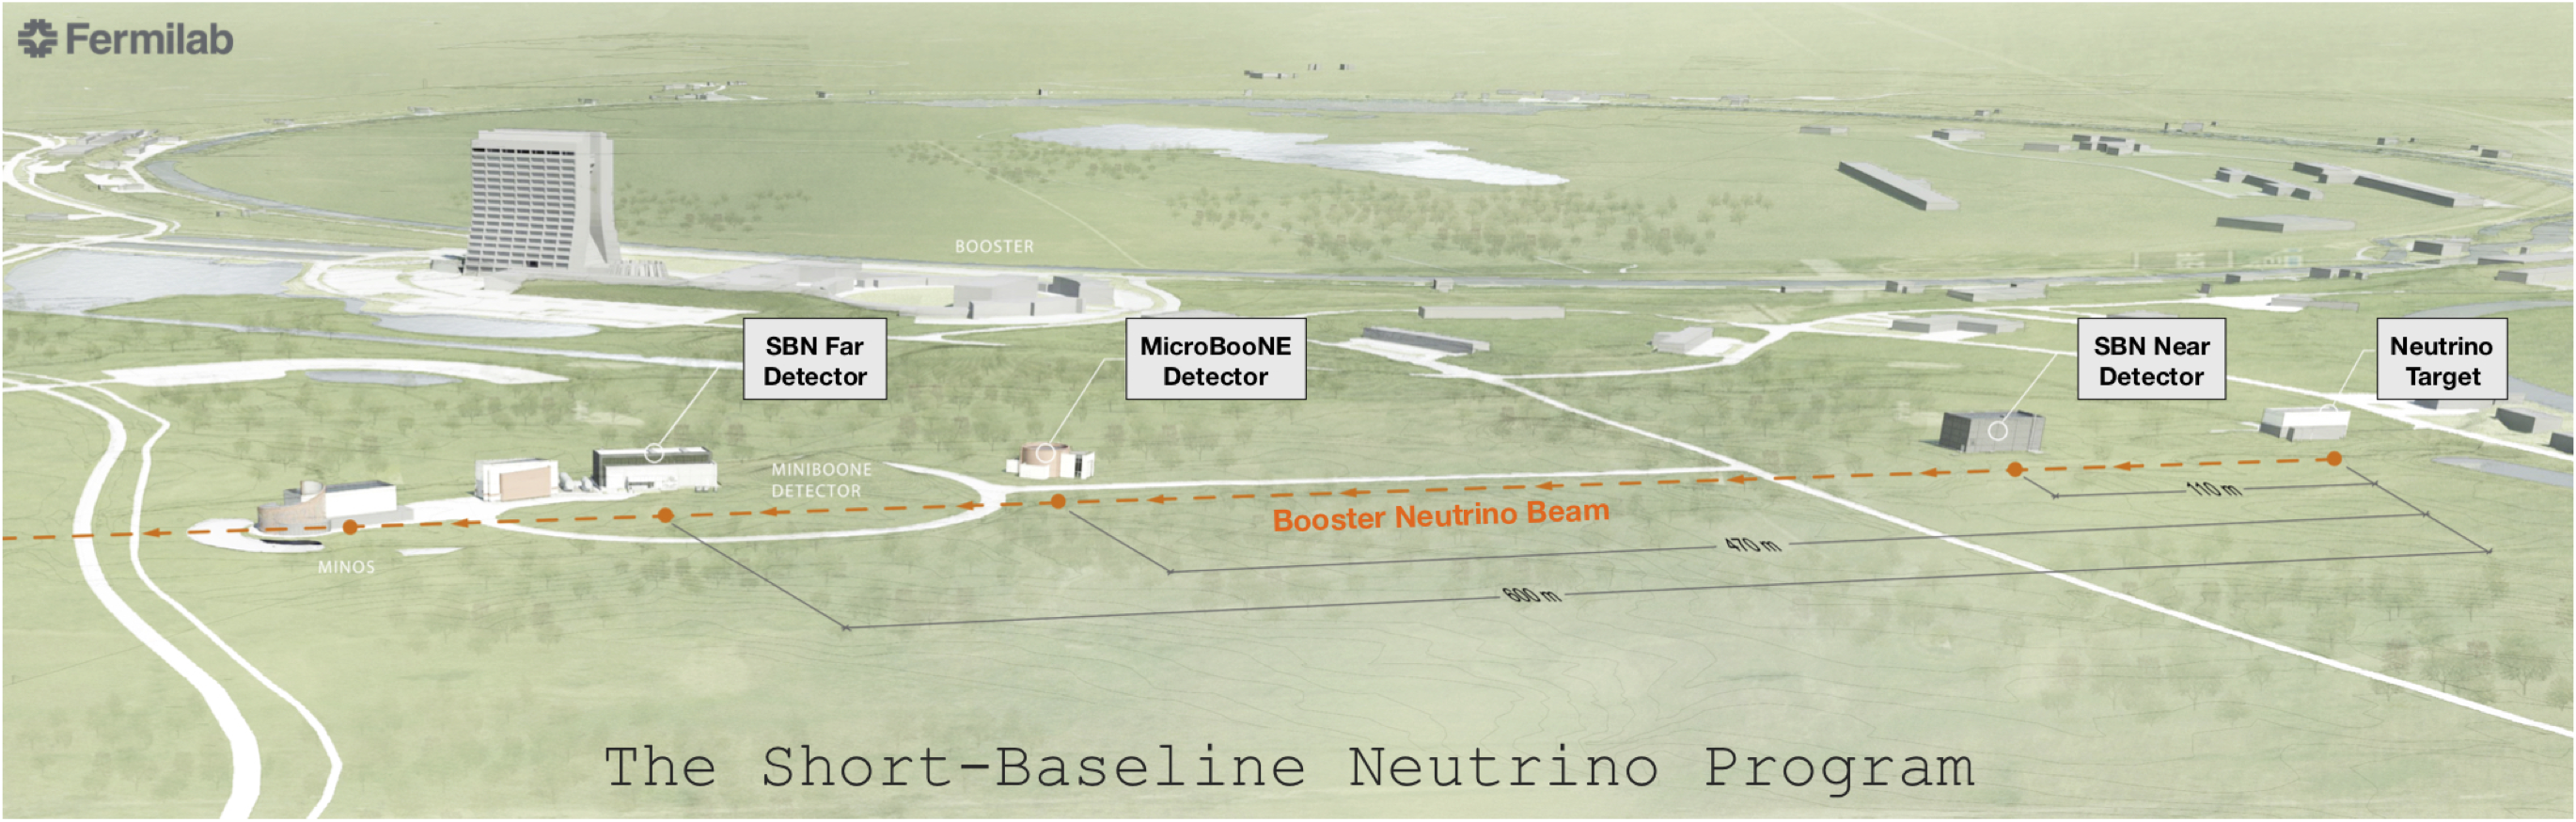
\includegraphics[scale=0.32]{Figures/SBN.png}
		\caption[The Short-Baseline Neutrino Program]{\textbf{The Short-Baseline Neutrino Program}\\The Short-Baseline Neutrino Program detectors as seen from an upper view at Fermilab. To the right is the neutrino beam target area where $8$ GeV protons from the Booster accelerator impinge a beryllium target. The beam is focused along the orange dashed line traveling toward the left (north). The SBND, MicroBooNE, and ICARUS \cite{SBN}.
		}
		\label{sbn_program}
	\end{center}
\end{figure}
%
The SBND is, as the name implies, the program's near detector and it consists of a $112$ton active mass LArTPC is at $110$ m from the target. It is currently under  installation phase and it is expected to be taking date mid-late next year,2023. In-between ICARUS and SBND, at $470$ m from the target, there is MicroBooNE, a $89$ton active volume LArTPC that has been taking da since 2015. Where each of the detectors are in the BNB beamline, at Fermilab, is illustrated in figure \ref{sbn_program}.
I will later describe in more details SBND and MicroBooNE, as they are the experiments in which I've carried my Ph.D. work. 
%
\section{The Deep Underground Neutrino Experiment}
%
The Deep Underground Neutrino Experiment (DUNE) is one of the most promising experiments for neutrino physics, as it aims to measure the CP violating phase in the leptonic sector, to determine the character of the neutrino mass spectrum, and to make precision measurements of oscillation parameters. Beyond the neutrino physics goals, DUNE also aims to search for baryon number violating processes and to perform precision measurements of neutrinos from a core-collapse supernova within the Galaxy, if one happens during the experiment's operating period. 
To accomplish such bold goals, DUNE designed with a near detector placed at Fermilab and a far detector at the Sanford Underground Research Laboratory in Lead, South Dakota. An intense neutrino beam of up to $2.4$ megawatts is produced at Fermilab, crosses the near detector, and travels $1,300$ kilometers downstream through Earth's crust to reach the far detector. In figure \ref{DUNE_full_schematic} you can see an schematic diagram of the experiment. 
%
\begin{figure}[h!]
	\begin{center}
		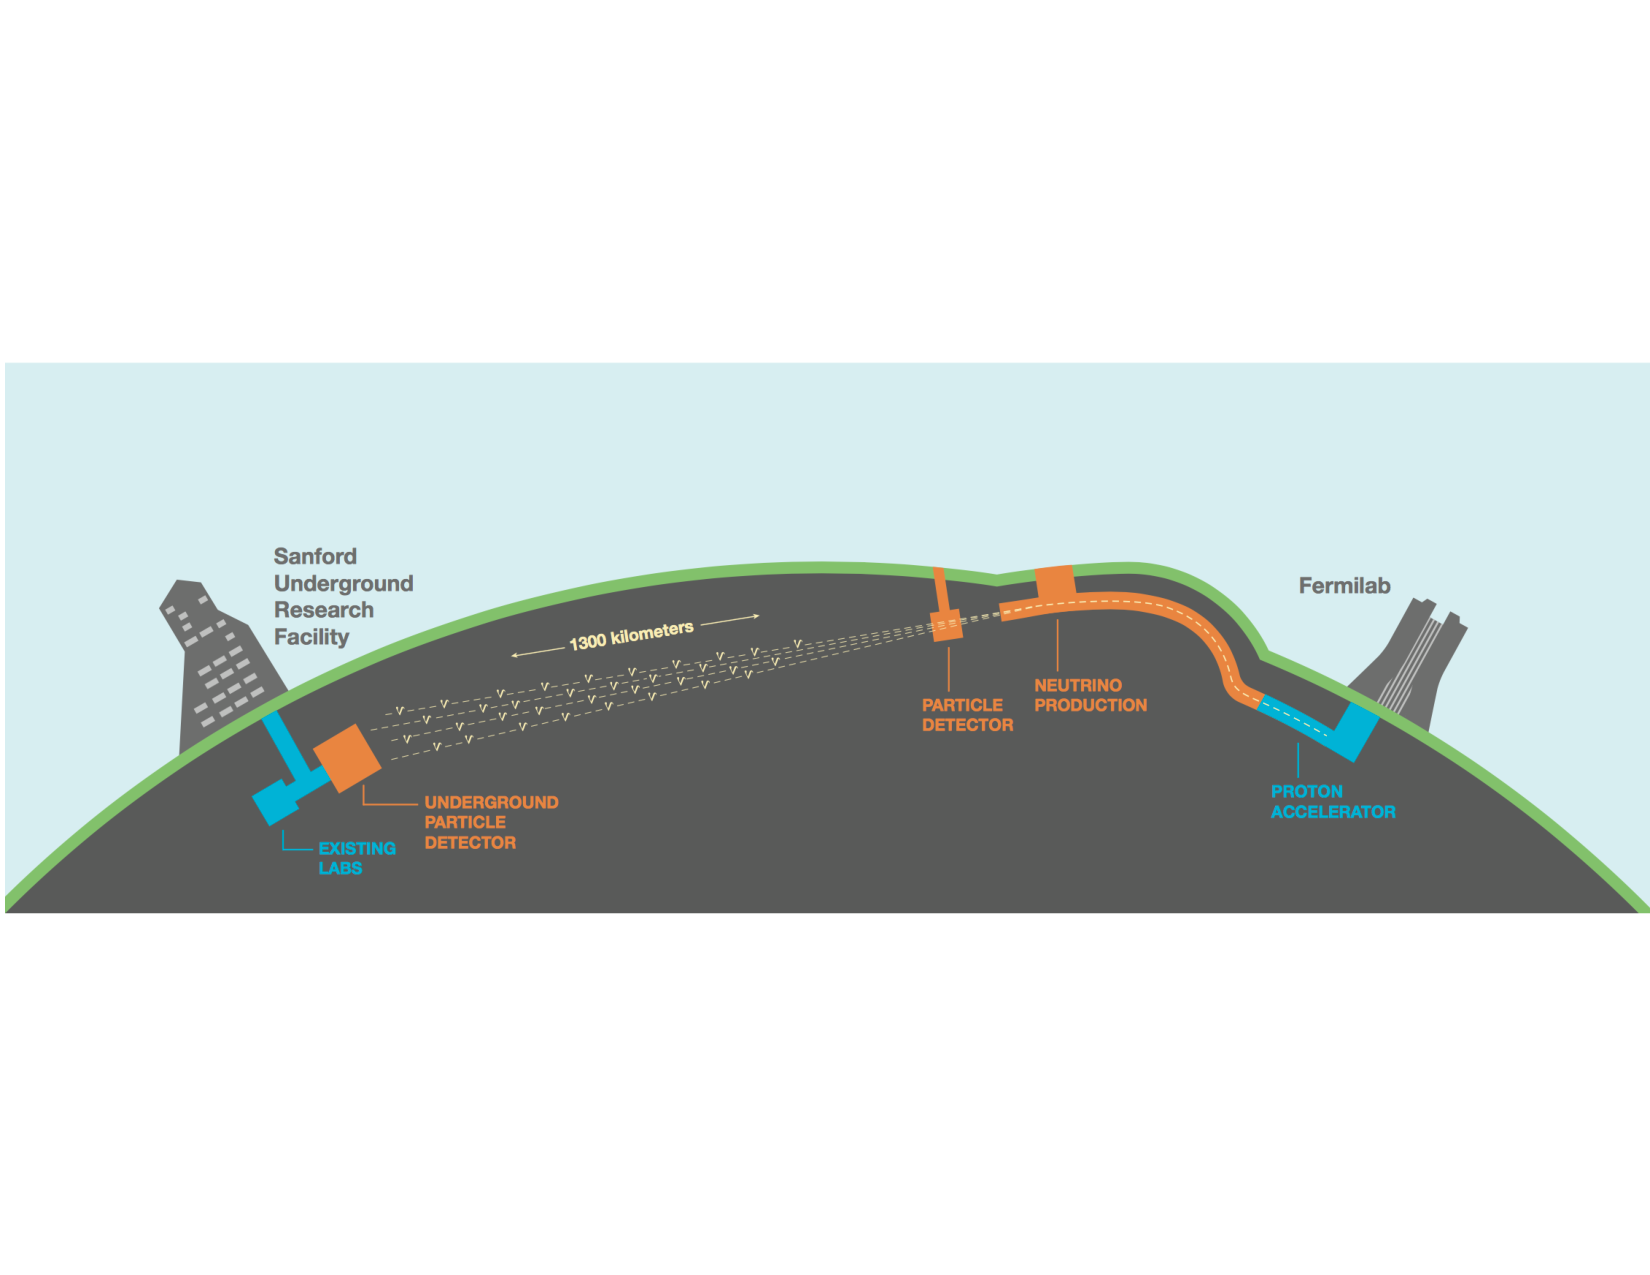
\includegraphics[scale=0.6]{Figures/DUNE_full_schematic.pdf}
		\caption[DUNE's full schematic]{ {\textbf{DUNE's full schematic.}} \\The figure shows the full DUNE's schematics, providing a view of the production of the neutrino beam, the Near Detector at Fermilab, the under crust travel of the beam, and the Far Detector at SURF \cite{dune_snowmass_22}.}
		\label{DUNE_full_schematic}	
	\end{center}
\end{figure}
%
DUNE's far detector is made of $4$ LArTPCs modules, of $10$ kton each. The near detector will have a combination of three different detection systems: a modular and optically segmented LArTPC of $\approx300$ tons (ND-LAr), a magnetized high-pressure Gas Argon Time Projection Chamber (GArTPC) surrounded by a calorimeterm (ND-GAr), a magnetized beam monitor consisting of an electromagnetic calorimeter, an inner target/tracker system and an active LAr target (SAND). \cite{dune_snowmass_22, dune_SAND}.